\documentclass{article}


% if you need to pass options to natbib, use, e.g.:
%     \PassOptionsToPackage{numbers, compress}{natbib}
% before loading neurips_2024

\PassOptionsToPackage{numbers, compress}{natbib}

% ready for submission
\usepackage{neurips_2024}
\bibliographystyle{abbrvnat}

\usepackage[pdftex]{graphicx}

% to compile a preprint version, e.g., for submission to arXiv, add add the
%[preprint] option:
%\usepackage[preprint]{neurips_2024}


% to compile a camera-ready version, add the [final] option, e.g.:
%     \usepackage[final]{neurips_2024}




\usepackage[utf8]{inputenc} % allow utf-8 input
\usepackage[T1]{fontenc}    % use 8-bit T1 fonts
\usepackage{hyperref}       % hyperlinks
\usepackage{url}            % simple URL typesetting
\usepackage{booktabs}       % professional-quality tables
\usepackage{amsfonts}       % blackboard math symbols
\usepackage{amsmath}
\usepackage{nicefrac}       % compact symbols for 1/2, etc.
\usepackage{microtype}      % microtypography
\usepackage{xcolor}         % colors


\title{SmokeViz: Using Pseudo-Labels to Develop a Deep Learning Dataset of Wildfire Smoke Plumes in Satellite Imagery}


% The \author macro works with any number of authors. There are two commands
% used to separate the names and addresses of multiple authors: \And and \AND.
%
% Using \And between authors leaves it to LaTeX to determine where to break the
% lines. Using \AND forces a line break at that point. So, if LaTeX puts 3 of 4
% authors names on the first line, and the last on the second line, try using
% \AND instead of \And before the third author name.


\author{%
    Rey Koki\(^{1,2}\)  \thanks{corresponding author: \texttt{rey.koki@colorado.edu} } \quad Michael McCabe\(^{1}\) \quad Dhruv Kedar\(^{1}\)\\ 
    \textbf{Christina Kumler-Bonfanti}\(^{1,2}\) \quad \textbf{Jebb Stewart}\(^{2}\) \quad  \textbf{Jed Brown}\(^{1}\) \\
    \(^1\)University of Colorado, Boulder \quad \(^2\)National Oceanic and Atmospheric Administration\\
  % Affiliation \\
  % Address \\
  % \texttt{email} \\
  % \AND
  % Coauthor \\
  % Affiliation \\
  % Address \\
  % \texttt{email} \\
  % \And
  % Coauthor \\
  % Affiliation \\
  % Address \\
  % \texttt{email} \\
  % \And
  % Coauthor \\
  % Affiliation \\
  % Address \\
  % \texttt{email} \\
}


\begin{document}


\maketitle


\begin{abstract}
The increase in the frequency of wildfires on a global scale underscores the need for advancements in fire monitoring techniques for disaster management, environmental protection and to mitigate negative health outcomes. This research introduces an innovative, data-driven framework that leverages the semi-supervised method, pseudo-labeling, to generate smoke plume annotations in geostationary satellite imagery. Unlike many pseudo-labeling applications that aim to increase the labeled dataset size, the primary objective is use pseudo-labels to refine an existing National Oceanic and Atmospheric Administration smoke dataset that provides temporal and geographical information on individual smoke plumes but at variable and, primarily, low temporal resolution. We use deep learning and pseudo-labels to pinpoint the singular, most representative, satellite image that optimally illustrates the smoke annotation within the given time window. By identifying the most representative imagery of smoke plumes for a given smoke annotation, the study seeks to create an accurate and relevant machine learning dataset. The resulting dataset is anticipated to be an instrumental tool in developing further machine learning models, such as an automated system capable of real-time monitoring and annotation of smoke plumes directly from streaming satellite imagery.
\end{abstract}


\section{Introduction}

In recent years, the escalation of wildfire incidents worldwide has become a prominent environmental and public health concern. The combustion process in wildfires releases smoke containing fine particulate matter (PM2.5) and harmful gases, posing severe hazards to human health and air quality. These risks underscore the necessity for efficient and effective monitoring methods to mitigate the adverse health impacts associated with wildfire smoke. 

Traditionally, wildfire monitoring has relied on ground-based methods, such as forest service patrols, manned lookout towers, and aviation surveillance \cite{smoke_monitoring}. While these methods provide valuable localized insights, they are constrained by geographical and logistical limitations, often failing to deliver timely and comprehensive data, especially over large and remote areas. In contrast, satellite imagery offers a vantage point that overcomes these limitations, providing continuous, wide-area coverage and real-time data crucial for assessing and responding to the health risks posed by wildfire smoke.

Satellite imagery, equipped with state-of-the-art sensors, such as the Advanced Baseline Imager (ABI) on the Geostationary Operational Environmental Satellites (GOES) \cite{goes}, have revolutionized environmental monitoring. These tools enable the detailed observation of smoke plumes, their particulate density, and the extent of smoke spread. These satellite-based systems offer the capabilities to provide critical insights into the concentration and movement of smoke particulates, facilitating real-time assessments of air quality.

The integration of satellite imagery in wildfire smoke monitoring is not only instrumental in providing real-time data but also plays a significant role in public health planning and response. By mapping the spread and density of smoke, health authorities can issue timely warnings, implement evacuation protocols, and deploy resources effectively to mitigate health risks. Furthermore, long-term data gathered from satellite observations can aid in understanding the broader impacts of wildfire smoke on public health, influencing policy decisions and preventive measures.

Currently, multi-channel thresholding is a popular method to distinguish smoke pixels from pixels containing dust, clouds or other phenomenon with similar signatures \cite{threshold}. Thresholds are determined by using historical, labeled data to extract optimal radiance values for each channel that corresponds with the labeled class. These methods are tuned to particular biogeographies and often have issues with generalization to new locations with varying fuel types \cite{thresh_geog}.

In contrast to the numerical thresholding approach, human visual inspection of satellite imagery is another commonly used method for smoke identification. Trained analyst inspect satellite imagery and label the smoke by hand. An example of hand-labeled annotations is the National Oceanic and Atmospheric Administration (NOAA) Hazard Mapping System (HMS) fire and smoke product \cite{hms, hms_val}. For the HMS smoke product, trained satellite analysts use movement characteristics to help identify smoke by scanning through a time series of satellite imagery. When visual inspection indicates smoke, the analyst will draw a polygon that corresponds to the geolocation and density of smoke. By design of the product, the HMS annotations have varying time resolution and are released on a rolling but undefined schedule ranging from one to multiple times a day as observation conditions permit. This method is potentially not as scalable as an automated approach and is limited by the availability of analysts and their time. 

To address the challenges associated with thresholding and manual labels, we can look towards innovative approaches and recent technological advancements in computer vision. Machine learning methods have shown potential in improving the accuracy and efficiency of satellite-based wildfire smoke detection and monitoring. For instance, SmokeNet, uses a convolutional neural network (CNN) based framework to determine if a scene of MODIS satellite imagery contains smoke \cite{smokenet}. Another study, that looked at a singular wildfire event, also used a CNN to identify smoke on a pixel-wise basis using imagery from Himiwari-8 \cite{larsen}. Additionally, Wen et al. developed a CNN architecture that takes GOES-East imagery as input and the HMS-generated annotations for the target labels during training \cite{smoke_goes}. 

The success of deep learning methods, such as CNNs, relies heavily on the availability of a large, representative dataset \cite{data_size}. As laid out in table \ref{studies}, prior studies use relatively small numbers of samples, from 47 \cite{wang} to 6825 \cite{smoke_goes}, where one sample represents a satellite image with a singular time and geolocation. In contrast, benchmark datasets for image classification contain tens of thousands (CIFAR-10 and MNIST) to millions (CIFAR-100 and ImageNet) of data samples \cite{cifar}, \cite{mnist}, \cite{imgnet}. Keeping in mind the correlation between both the quality and quantity of data with model performance, we introduce the largest known smoke dataset, SmokeViz, containing over 130,000 samples.

\begin{table}[h]
    \caption{Comparison of different studies including method used, dataset size, satellite source, number of channels used and if classification is performed at a pixel or image level.}\label{studies}
    \centering
    \begin{tabular}{ccccrrcrc}
        \toprule
        Reference & Method & \verb|#| Samples & Satellite & \verb|#| Channels & Level\\
        \midrule
        \cite{smokenet}& CNN & 6255 & MODIS & 5 & image\\
        \cite{smoke_goes}& CNN & 6825 & GOES-East & 5 & pixel\\
        \cite{larsen} & CNN & 975 & Himiwari-8 & 7 & pixel\\
        \cite{wang}& U-Net & 47 & Landsat-8 & 13 & pixel\\
        SmokeViz  & U-Net & 133,871 & GOES-East/West & 3 & pixel\\
        \bottomrule
    \end{tabular}
\end{table}


Semi-supervised learning is an approach that can be used to increase the number of labeled samples in a dataset. This is done by leveraging a labeled dataset to generate new labels for an often larger, but unlabeled, dataset. Pseudo-labeling, a form of semi-supervised learning, uses labeled data to train an initial model, then runs that model on unlabeled data to predict pseudo-labels, and finally trains a new model using the pseudo-labels \cite{pseudo}. We introduce a variation of pseudo-labeling, not to increase the size, but to increase the quality of our dataset by using pseudo-labels to select the best satellite image out of a given time-window to represent each smoke plume annotation.


\section{Methods}
\subsection*{Dataset}

The initial data source, discussed in further detail in the HMS Smoke Labels section, is uniquely characterized by each annotation having corresponding imagery ranging between 1-60 frames, where each frame captures 5 minutes of exposure.  Additionally, we have two satellites that overlap in coverage area, GOES-East and GOES-West, effectively doubling the number of frames for a single annotation. We apply pseudo-labeling to develop a dataset that has a one-to-one annotation-to-image ratio, where we choose the satellite image that has the maximum overlap between the geolocation of smoke in the imagery and the analyst annotation.

Dataset development came in three stages. First, we leverage light scattering physics to determine which singular satellite image would be in the optimal configuration for smoke detection. Second, we used that dataset to train an initial parent model that will identify smoke in satellite imagery. Third, we use that parent model to label each satellite image in a given annotation's time-window and the optimal satellite image is chosen based on which image's pseudo-labels has the greatest overlap with the analyst annotation for the given location and densities of smoke.

\subsubsection*{HMS Smoke Labels} 
NOAA manages environmental satellite programs such as the HMS program, the HMS program is an operational system that uses an aggregation of satellite data to generate active fire and smoke data. To train our model, we implement a supervised learning framework that uses the HMS analyst smoke product as truth labels during the model training process.

HMS smoke analysis data gives the coordinates of the smoke perimeter as a polygon and classifies the smoke by density within a given time window. The time windows can range from instantaneous (same start and end time) to lengths of 5 hours. While the true bounds of the smoke can change within the larger time spans, the analyst is making an approximation that should reflect the smoke coverage over the duration of the time window. The density information is qualitatively determined by each analyst based on the apparent smoke opacity in the satellite imagery and categorized as either light, medium or heavy as seen in figure \ref{densities}a \cite{hms_web}.

\begin{figure}
    \centering
    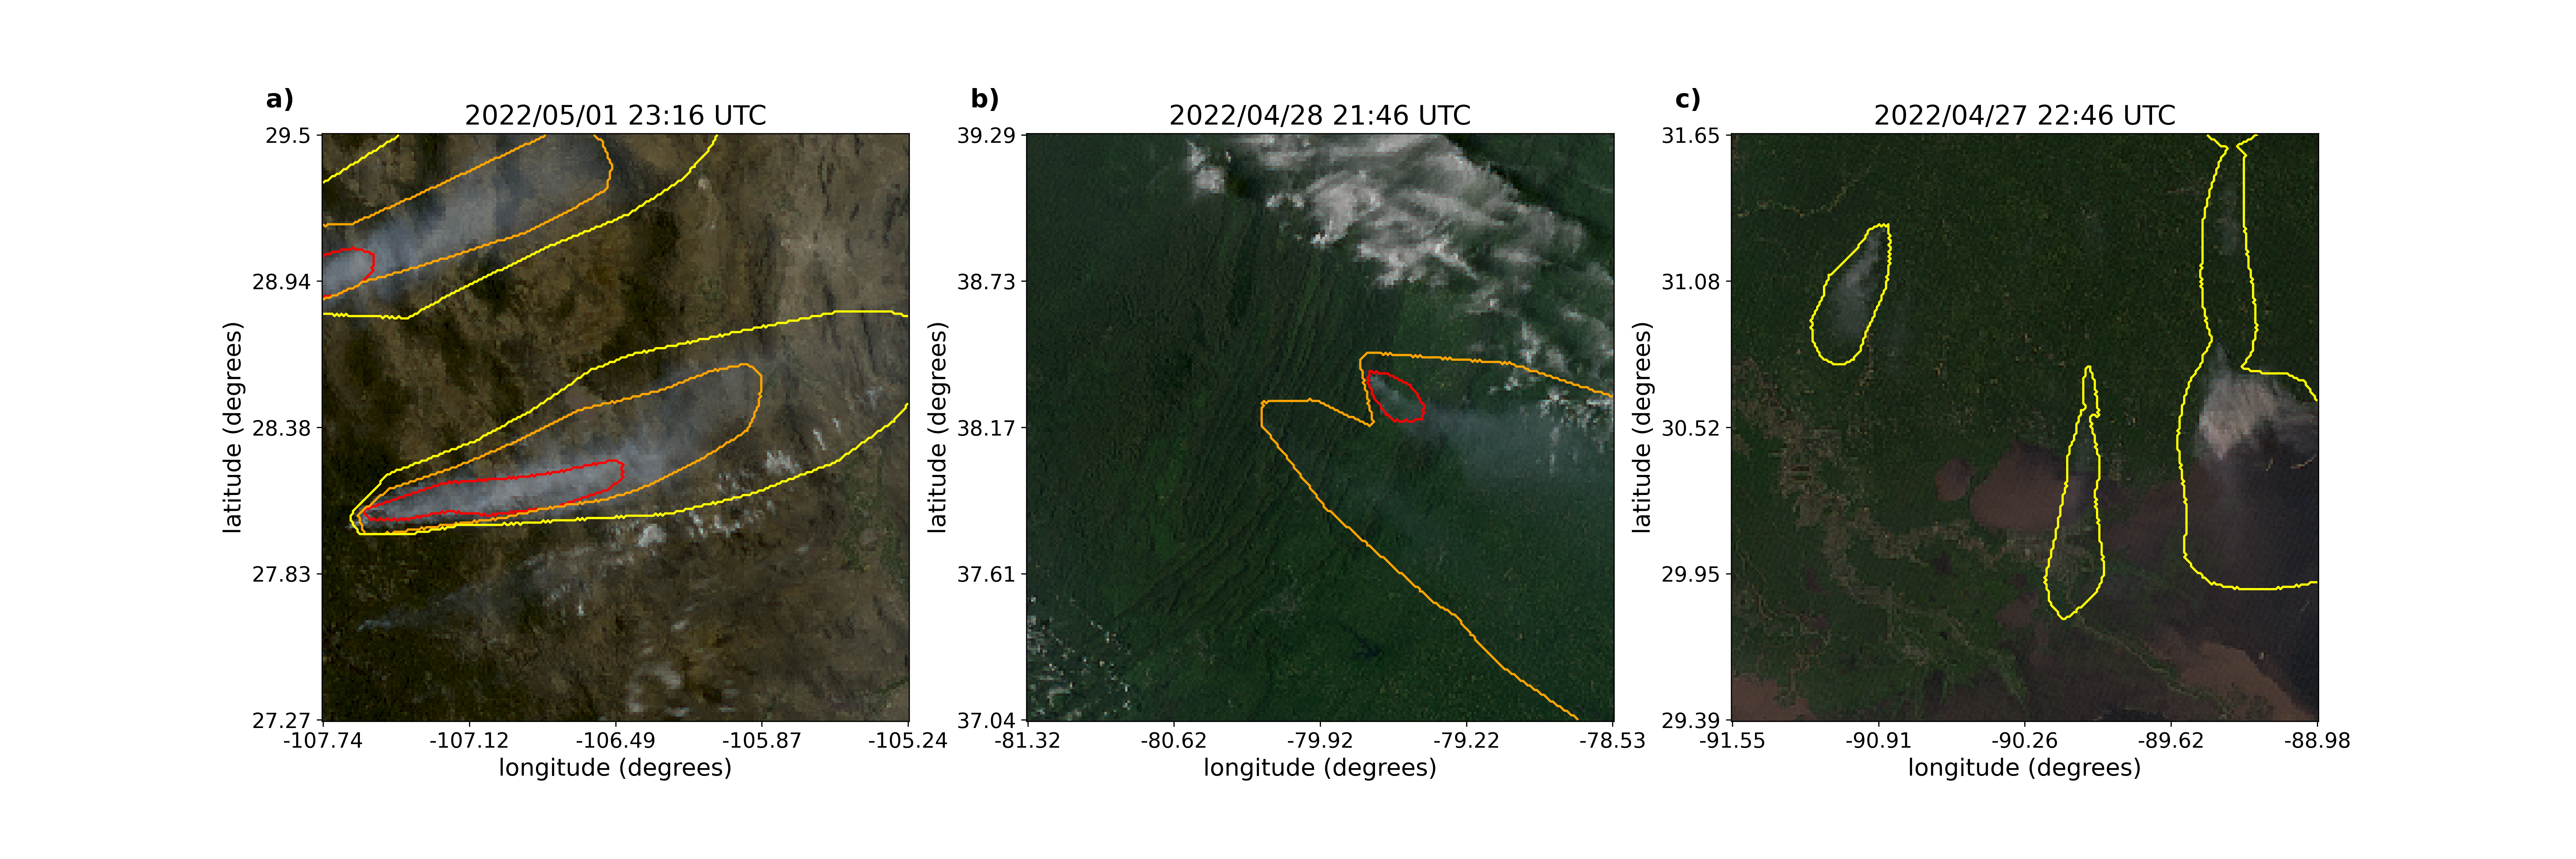
\includegraphics[width=14cm]{figures/Misclassified.png}
    \caption{Satellite imagery captured by GOES-East within a few days of each other. The yellow, orange and red contours indicate the extent of Light, Medium and Heavy smoke.  a) shows a canonical example of a smoke plume. b) and c) show observable variations in the density labels.}\label{densities}
\end{figure}

\subsubsection*{Thermometer Encoding Smoke Densities}

One of the challenges introduced with using human generated qualitative smoke densities was that, as seen in figure \ref{densities}b and \ref{densities}c, there are variations in what is labeled as heavy or light density smoke. More generally, reproducing qualitative metrics with quantitative algorithms is a challenging problem, but we apply mathematical approaches that mitigate some of the underlying complications of our specific problem. Despite the fact that the smoke densities introduce qualitative complexities, we decided that the density approximations were important to use in our dataset because of the differences in signatures the densities produce. Within the satellite imagery, the appearance of a light density smoke plume will look significantly different than a heavy density smoke plume as seen in figure \ref{densities}. Additionally, a light density smoke plume is expected to be more challenging to detect since it is easier for it to be misclassified as not smoke. During the training process, the separate density categories allows us to deferentially weight the penalization given to the model for incorrect classifications based on category. For example, the model can be given a small penalization for misclassifying light smoke as not smoke while given a higher penalization for misclassifying heavy smoke as not smoke. 

In addition to the densities being ordered and categorical, the differences between the density categories are not evenly distributed by a given metric, such as particulate matter per square meter. The intervals between densities being unknown along with the hierarchical nature of the density labels makes the labels ordinal instead of just categorical. This data property allows us to use thermometer encoding \cite{therm_enc}, which leverages the idea that heavy density smoke includes both medium and light density smoke, that heavy density smoke is closer to medium than it is to light, and automatically weights the loss functions and incorporates the ranked ordering of the densities.  As seen in Table \ref{therm}, one-hot encoding, commonly used for categorical data, doesn't take ordinal properties of the data into consideration.  

\begin{table}[h] 
    \caption{A comparison of one-hot encoding used for categorical data to thermometer encoding for ordinal data.}\label{therm}
    \centering
    \begin{tabular}{ccccrrcrc}
        \toprule
        category & one-hot & thermometer \\
        \midrule
        No Smoke & \texttt{[0 0 0]} & \texttt{[0 0 0]} \\
        Light  & \texttt{[0 0 1]} & \texttt{[0 0 1]} \\
        Medium & \texttt{[0 1 0]} & \texttt{[0 1 1]} \\
        Heavy  & \texttt{[1 0 0]} & \texttt{[1 1 1]} \\
        \bottomrule
    \end{tabular}
\end{table}

\subsubsection*{Time Windows For Smoke Annotations}

In order to take into account movement characteristics to help identify smoke, analysts use multi-frame animations of the satellite imagery. The resulting annotations often have large time windows over multiple hours to represent one smoke plume annotation. Since the goal of these annotations is to show the general coverage over that time span, as shown in figure \ref{timelapse}, the smoke boundaries don't often match up with the satellite imagery over the entire time window. One way to approach this problem would be to use all the satellite images the analysts used as input. Since the timespans are non-uniform, this would vary the length in imagery inputs into the model, which would be difficult with a CNN architecture. Moreover, this would require a large amount of additional memory and computational resources. Instead of using the original analysts' many satellite image inputs to one annotated output, we develop a one-to-one input-to-output by finding the optimal singular satellite image input to represent the annotation. Discussed in further detail in the next section, we do this by making physics-driven choices on which satellite and timestamp would give the optimal angle between the sun and satellite that would produce the strongest smoke signature for the geolocation and timestamp of the smoke plume.


\begin{figure} \label{timelapse}
    \centering
    \includegraphics[width=13cm]{figures/timelapse.png}
    \caption{True color GOES-East imagery from May 2022, Southeast New Mexico (\(31^{\circ}\)N, \(100^{\circ}\)W) during the start of the Foster Fire. The red, orange and yellow lines represent the heavy, medium and low density HMS smoke annotations that span 19:10\textendash23:00 UTC.}
\end{figure}


\subsubsection*{Satellite Imagery} 

The GOES satellites are operated by NOAA in order to support meteorology research and forecasting for the United States. We use the latest operational satellites, GOES-16 (East), 17 and 18 (West) that each carry the ABI, that measure 16 bands between the visible and infrared wavelengths. In improvement to the GOES predecessors, imagery is collected every 5 minutes for the contiguous United States and every 10 minutes for the full disk. Using PyTroll, a Python framework for processing satellite data \cite{satpy}, we input bands 1-3 (Table \ref{rgb_bands}) to a GOES true color composite algorithm to develop a true color image representation \cite{true_color}, similar to what is seen by HMS analysts.

\begin{table}
    \caption{To create a true color image, we use the following bands from the ABI Level 1b CONUS (ABI-L1b-RadC) product.}\label{rgb_bands}
    \centering
        \begin{tabular}{ccccrrcrc}
            \toprule
            band & description & center wavelength ($\mathrm{\mu m}$) & spatial resolution (km)\\
            \midrule
            C01 &  blue visible & 0.47 & 1 \\
            C02 & red visible & 0.64 & 0.5 \\
            C03 & veggie near infrared & 0.865 & 1 \\
            \bottomrule
        \end{tabular}
\end{table}


\subsubsection*{Mie-Derived Dataset}

We used a physics-informed approach in selecting the initial dataset, \(\mathcal{D}_M\), which we call the Mie-derived dataset, for training an initial parent model, \(f_p\). Prior GOES ABI datasets for machine learning applications often include data from only one of the two GOES-series satellites, commonly opting for GOES-East \cite{smoke_goes}, \cite{wildfire_detect}, \cite{goes_conv}. Rather than using one satellite or the cumulative data from both GOES-West and GOES-East images, we select between one or the other based on the solar zenith angle. For smoke identification, this approach can achieve a much higher signal-to-noise than imaging the earth’s surface from an arbitrary angle. The elastic scattering of light is the primary mechanism to account for - while the atmosphere is composed of molecules with size \(<\)1nm, smoke particles can vary from 100 nm -- 10 \(\mu\)m in diameter, \(d\). The GOES ABI covers spectral bands from 0.47 \(\mu\)m -- 13.3 \(\mu\)m, so atmospheric and smoke particle sizes occupy two very different regimes with respect to the imaging wavelength \(\lambda\). In the extreme limit of \(\lambda \gg d\), the physics of scattering of light off a small sphere is captured by Rayleigh scattering. This process has two critical consequences: (1) the scattering cross section of light is strongly wavelength dependent (scaling with \(\lambda^{-4}\)), meaning that photons with wavelength closer to the ultraviolet are scattered more strongly than infrared photons. (2) the scattering cross section scales with an angular dependent cross section of \((1 + \cos^2 \theta)\). Scattered photons follow the emission distribution of a radiating dipole, scattering more strongly in the forward and backwards directions \((\theta = 0,\pi)\)than orthogonal to the direction of propagation \((\theta = \pi/2, 3\pi/2)\), see figure \ref{mei} for a Rayleigh scattering schematic.

%\begin{figure}
%    \centering
%    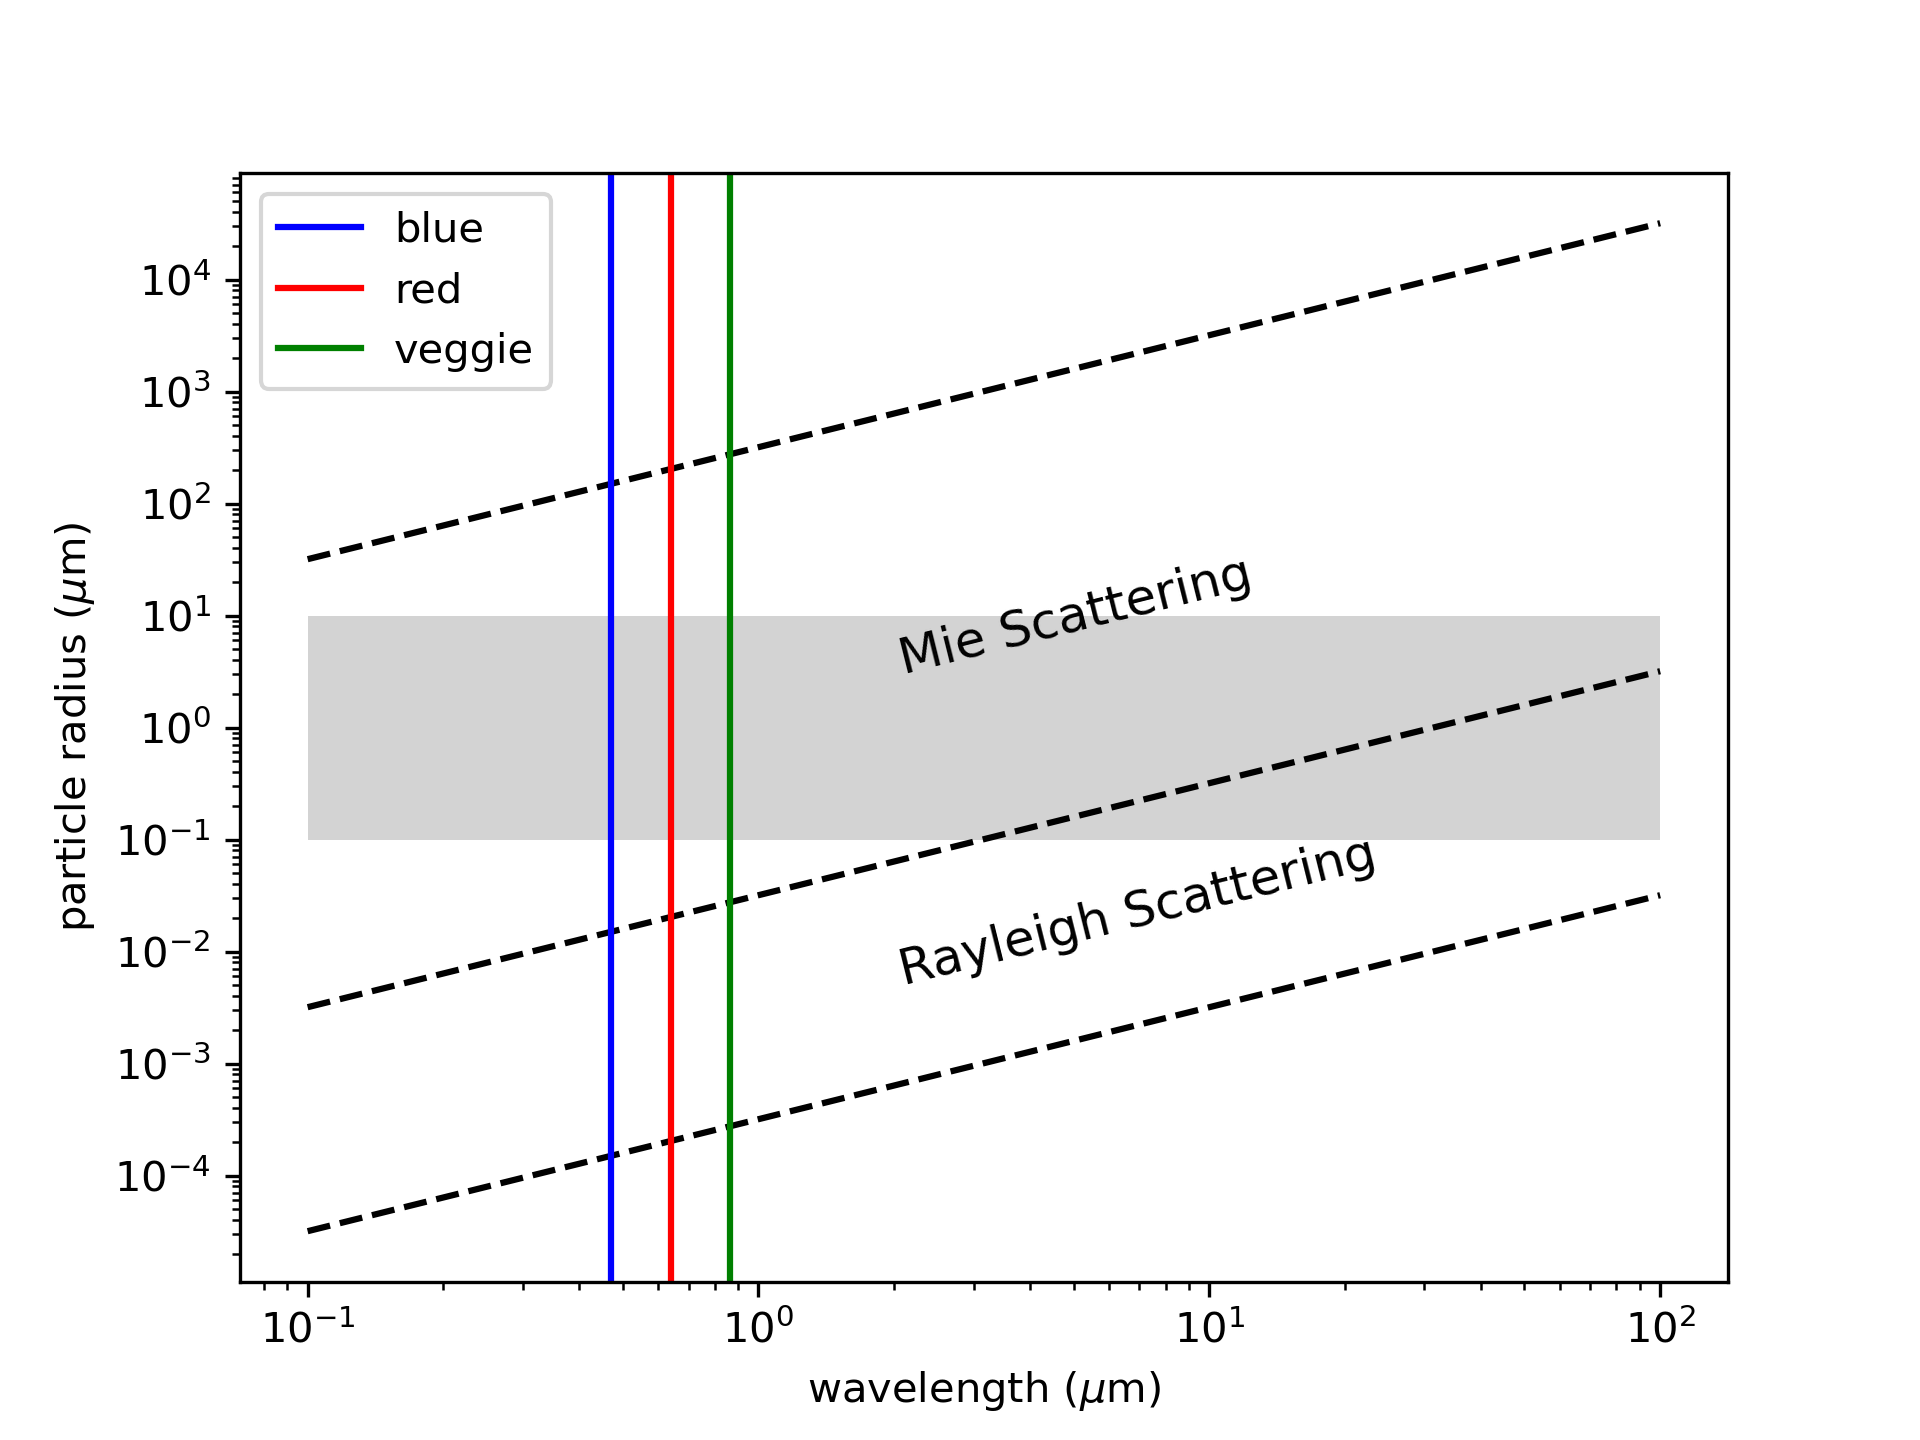
\includegraphics[width=10cm]{figures/scatter_regime.png}
%    \caption{Relationship between the size of a particle, the wavelength of light interacting with the particle and the type of scattering behavior induced by that interaction. The dotted lines represent rough estimates of the boundaries between the scattering regimes \cite{petty}. The gray area represents the range of particle radius relevant to smoke particulate matter.}\label{regime}
%\end{figure}

\begin{figure}
    \centering
    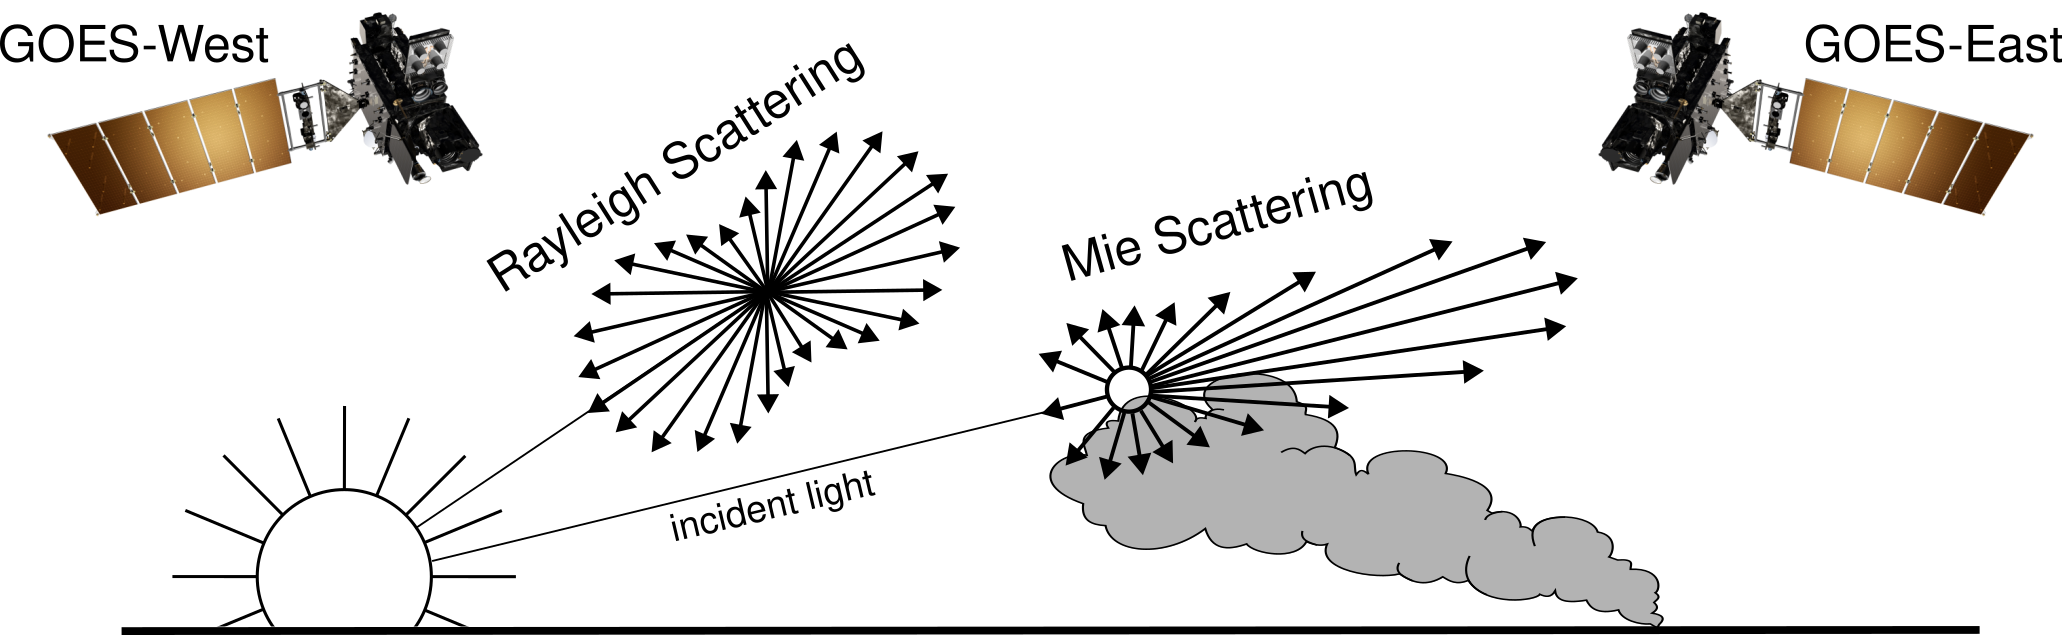
\includegraphics[width=10cm]{figures/mei.png}
    \caption{If the particle size is \(<\frac{1}{10}\) the wavelength of the interacting light, then the primary scattering will be Rayleigh. Mie scattering is the predominant scattering mechanism when the particle size is larger than the wavelength of light. This schematic demonstrates that when the sun is setting in the West, the Mie scattering will predominately forward scatter towards GOES-East.} \label{mei}
\end{figure}

The significance of these scalings is that the observer, or detector, will receive blue photons in most directions orthogonal to the source. Equivalently, photons traveling colinearly with line of sight to the emission source will mostly have wavelengths in the infrared band.  In the converse regime of \(d > \lambda\), the elastic scattering of light against matter is modeled through Mie scattering. In comparison to Rayleigh scattering, Mie scattering is largely wavelength-independent and has a more complicated radiation pattern where the cross section has a maximal amplitude in the forward direction. An observer downstream of this scatterer will collect more photons than one positioned directly behind it. In the context of smoke identification, a sunrise or sunset will lead to a higher Mie scattered signal in GOES-West and GOES-East respectively, as shown with a smoke plume producing a stronger signal in GOES-East imagery near sunset in figure \ref{16_vs_17}.

\begin{figure}
    \centering
    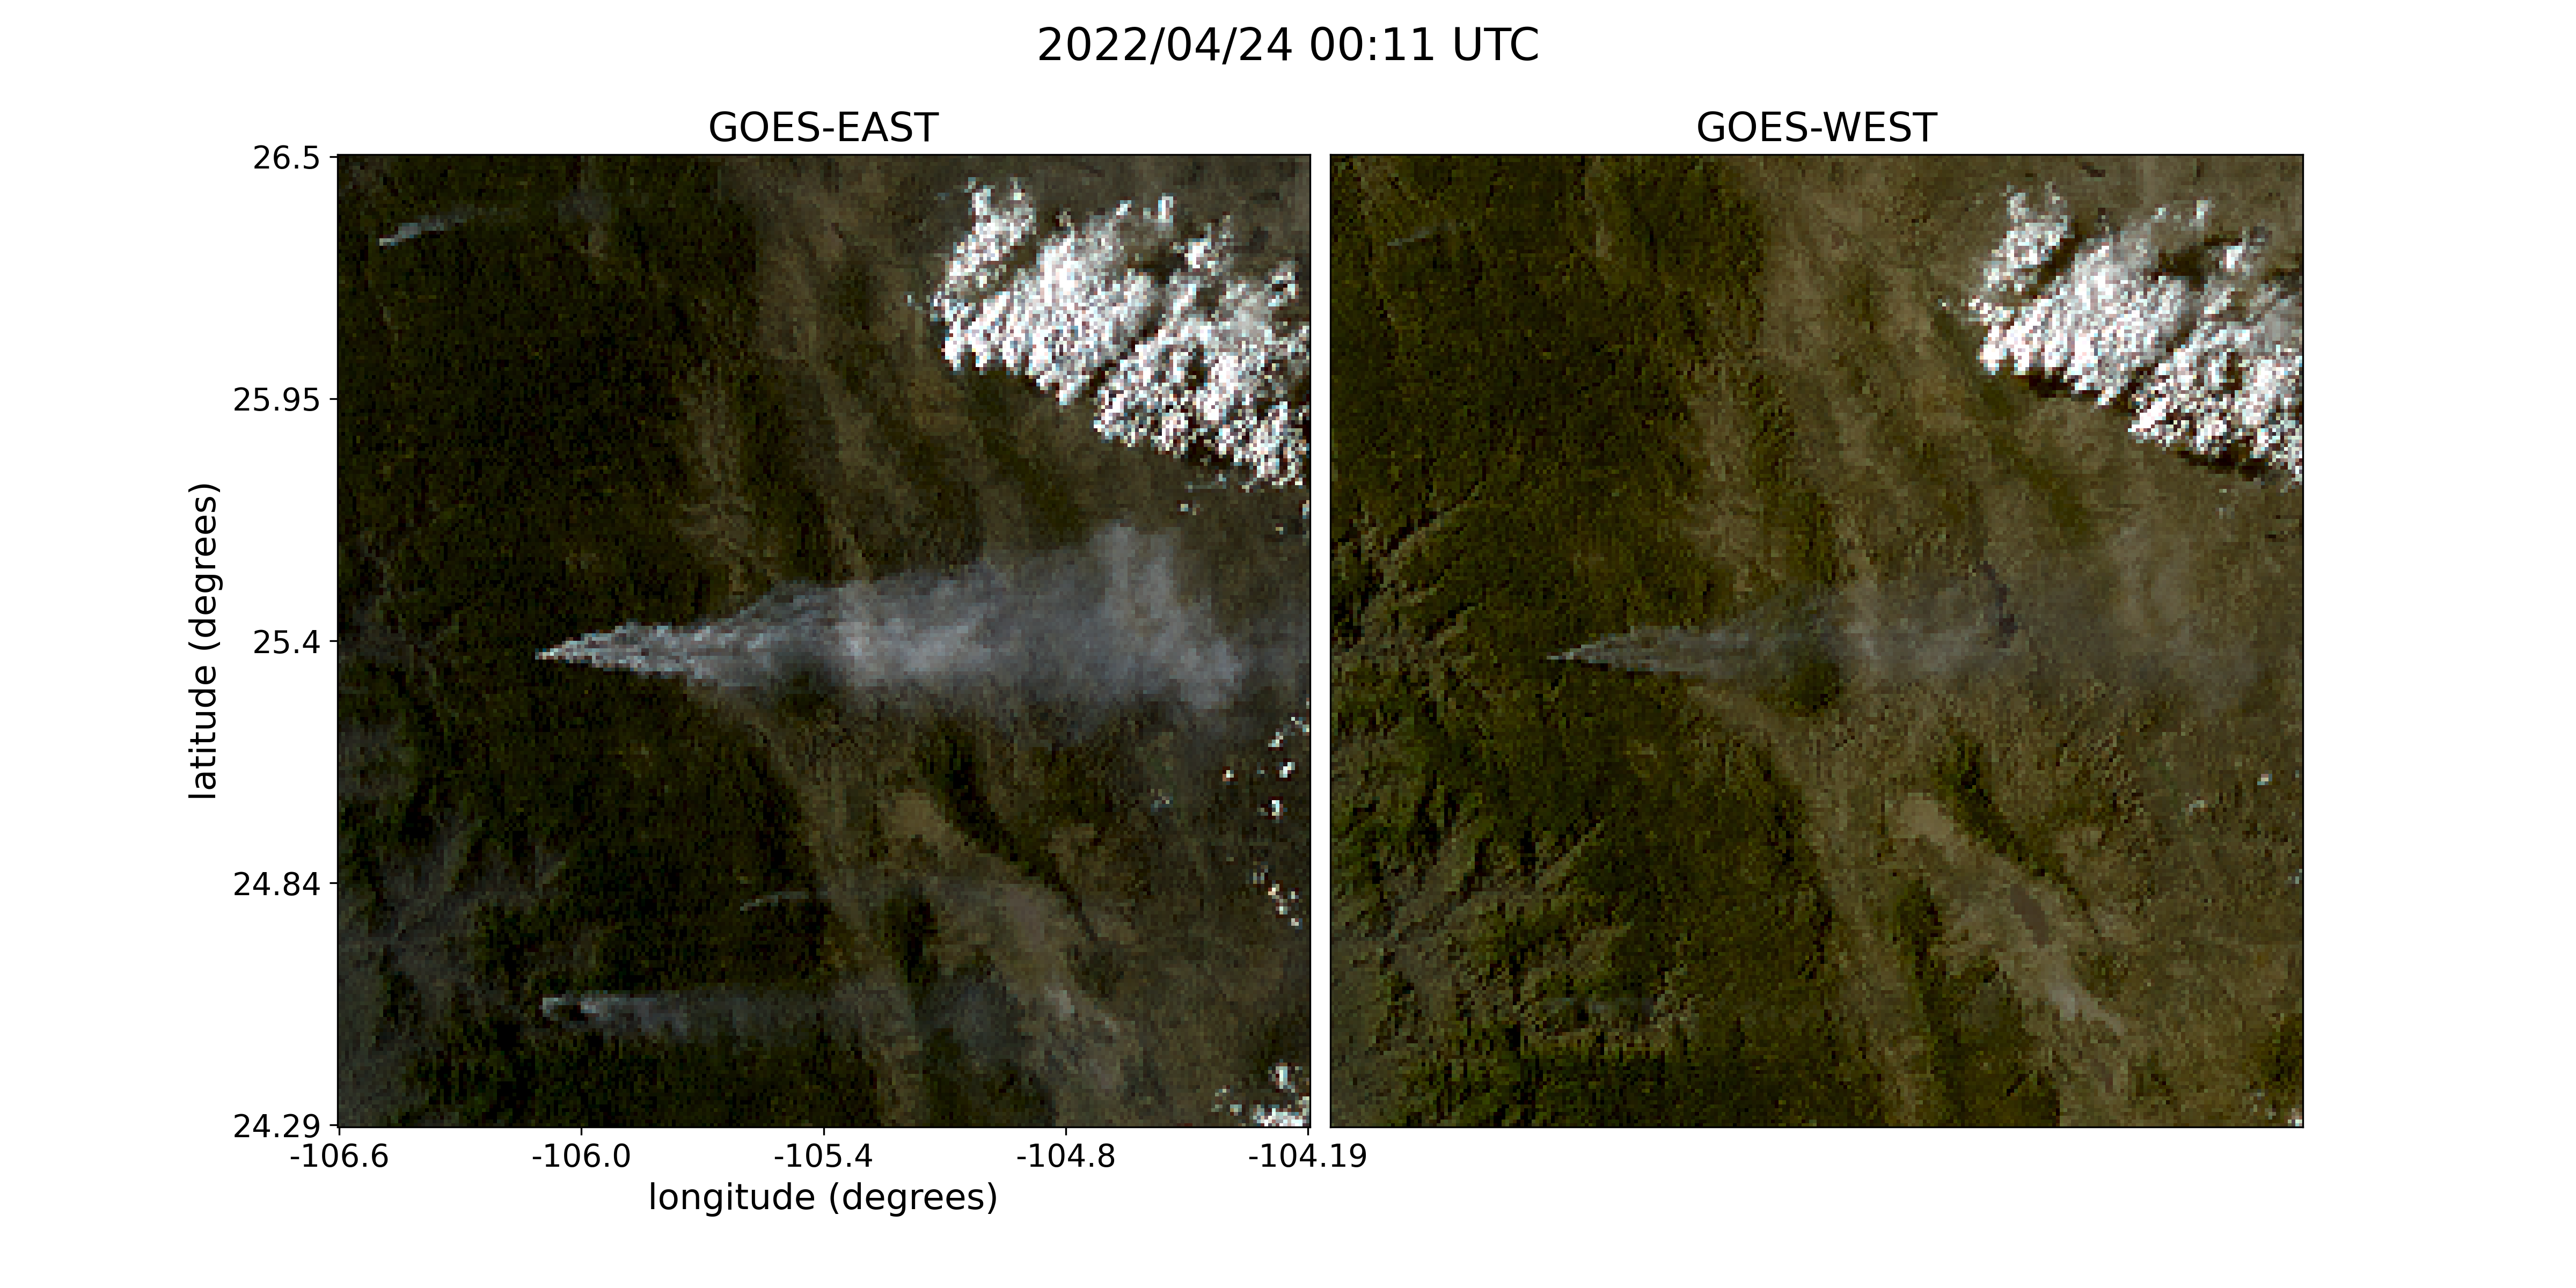
\includegraphics[width=12cm]{figures/G16_v_G17.png}
    \caption{True color GOES-East (left) and GOES-West (right) imagery from April \(24^{th}\), 2022 in Durango, Mexico. The images were taken \(\sim0.5\) hours before sunset (01:43 UTC) for this geolocation and time of year.}\label{16_vs_17}
\end{figure}

Smoke identification therefore amounts to extracting a signal of \(d > \lambda\) photons from the \(\lambda \gg d\) background. Positioning a detector along line of sight to the scatterer will result in a higher signal from smoke particles (figure \ref{mei}). Filtering the imaged wavelength can enhance this signal; photons collected in the blue spectrum will have a naturally lower background along the line of sight to the illumination source do their high level of Rayleigh scattering as. Therefore, as demonstrated in figure \ref{bands}, this configuration results in the highest signal to noise imaging for smoke particles.   

\begin{figure}
    \centering
    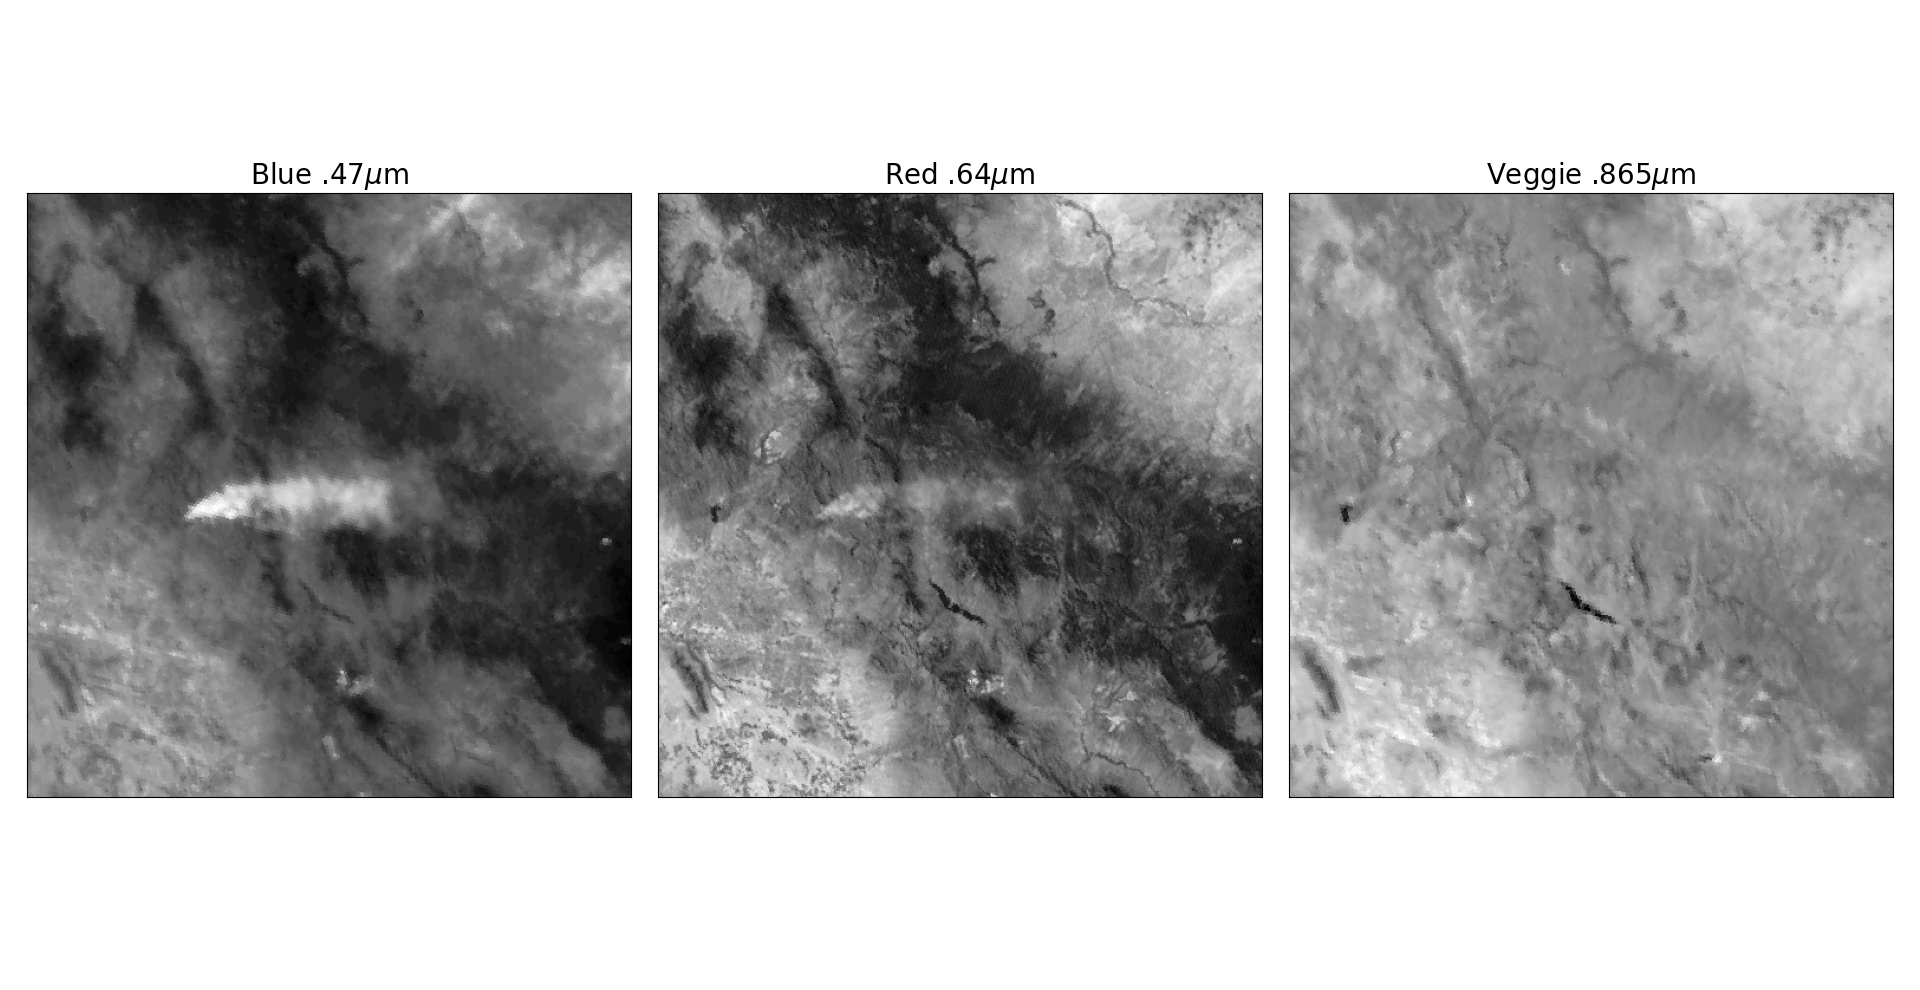
\includegraphics[width=10cm]{figures/GOES16_bands.png}
    \caption{Three bands of GOES-East data are the raw input to generate a true color image. These plots show variations in the signal-to-noise ratio for smoke detection in relation to the wavelength, \(\lambda\), of light being measured.}\label{bands}
\end{figure}

Based solely on these criteria, the optimal strategy would be to pull data from GOES-West right after sunrise and from GOES-East right before sunset. Another factor to consider is that the time when the sun is in optimal alignment with the satellite for smoke detection coincides with when solar zenith angle is maximized. Larger angles between the satellite and sun result in an increase in noise due to increased atmospheric interactions \cite{zen_angle}.  This is shown in figure \ref{G17_sunrise}, while we optimize for smoke signal detection, due to the high solar zenith angle, we introduce atmospheric interaction noise that obfuscate the smoke signal. To reduce the noise from large solar zenith angles, if given multiple options to choose from, we choose the image with the largest solar zenith angle that is below 80 degrees.

The resulting image selection process takes into account atmospheric properties and light scattering physics to generate an estimate of which singular satellite image within the analyst time-window could give the highest smoke signal-to-noise ratio. The resulting Mie-derived dataset, \(\mathcal{D}_M\), was then used to train a model, \(f_p\), that would generate \(N\) pseudo-labels, \(l^*\), for every sample, where \(N\) is determined by how many images, taken at a 10 minute interval, fit within the analyst time-window for that sample. Chosen from the \(N\) images, \(x^*\) is the image with the highest alignment between the \(f_p\) prediction of smoke, \(l^*\), in the image and the HMS analysts' annotation \(y^{a}\).

\begin{figure}
    \centering
    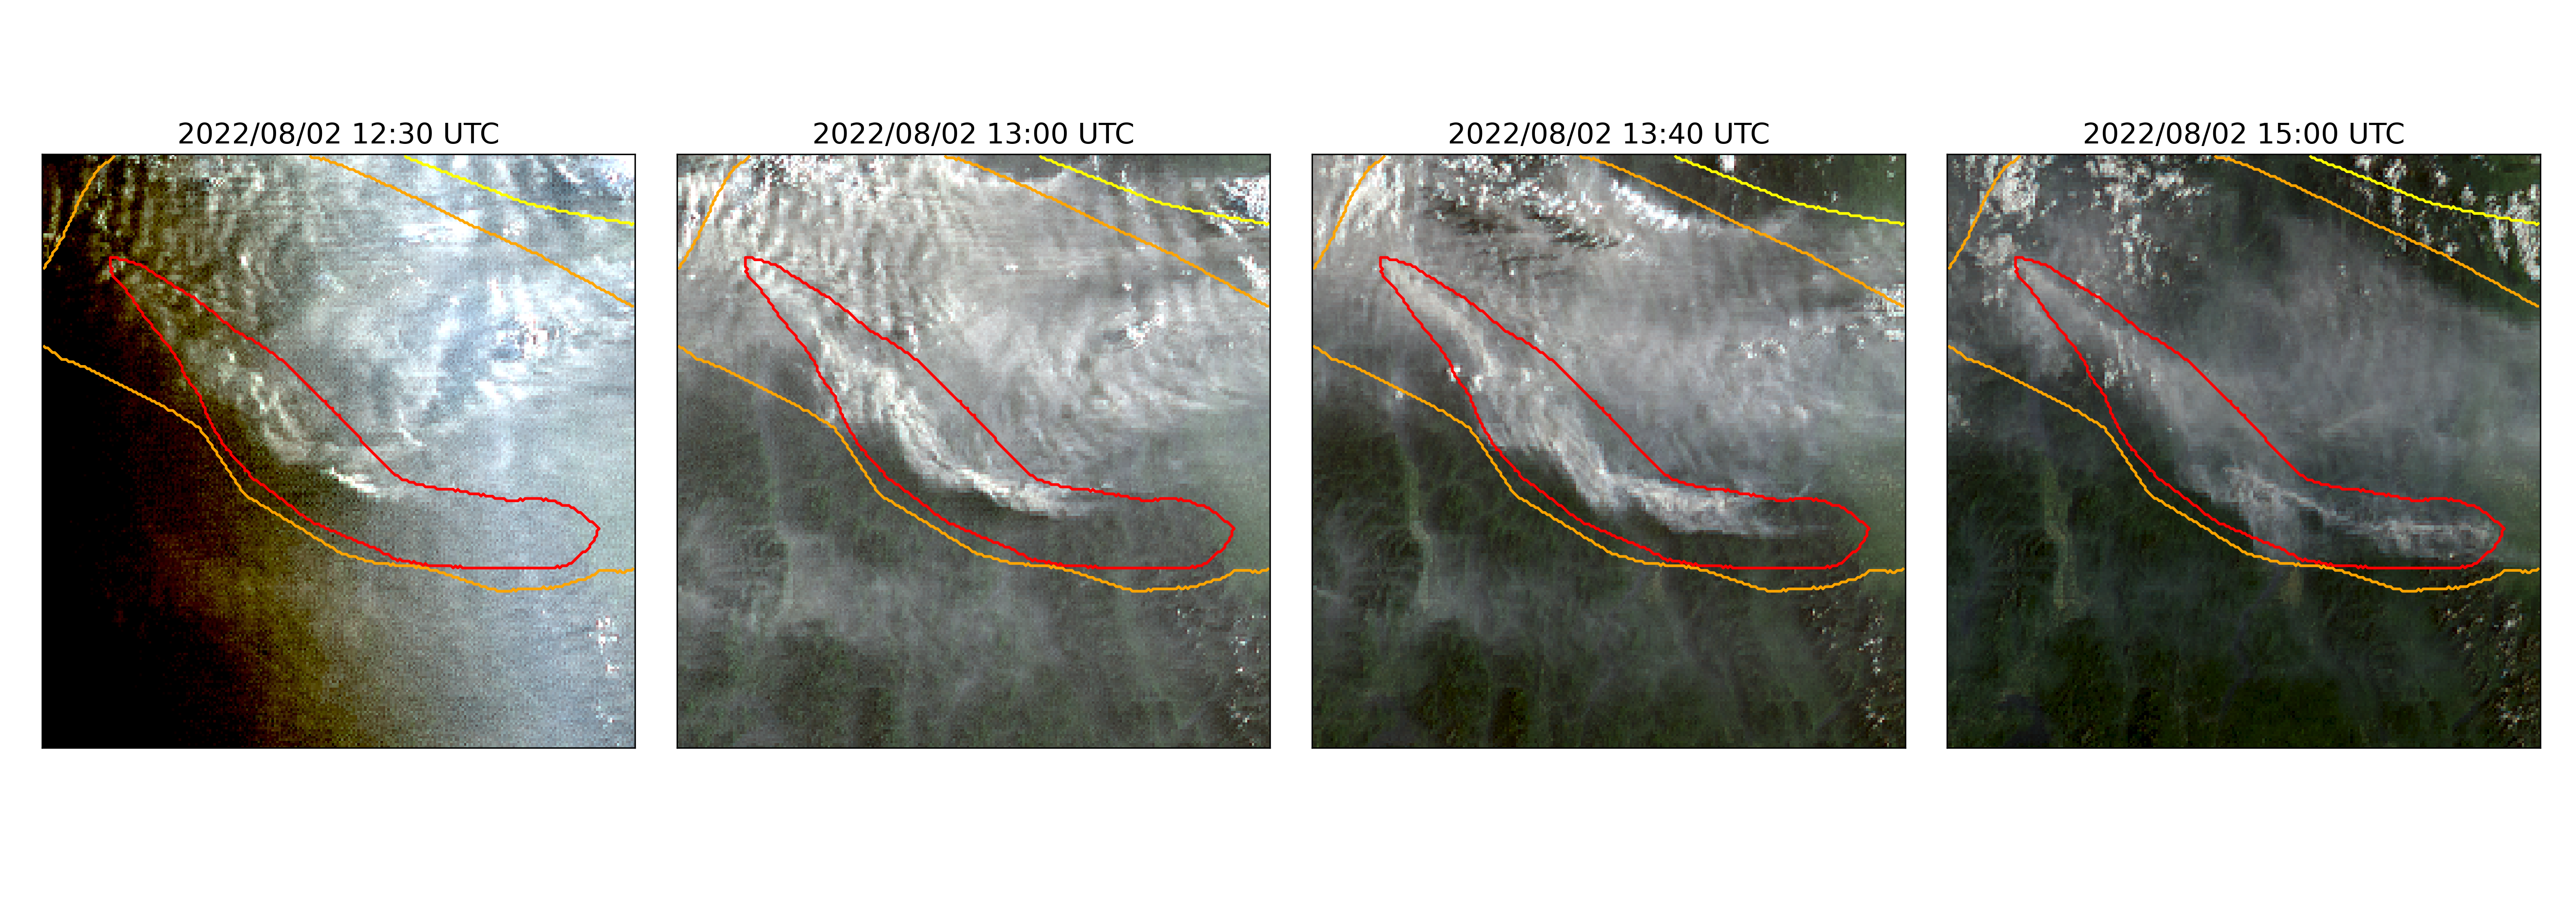
\includegraphics[width=12cm]{figures/timelapse_G17_2.png}
    \caption{A smoke annotation projected onto GOES-West imagery from August 2022 that spans from 11:00 UTC to 15:00 UTC, sunrise on August 2nd, 2022 at coordinates (49°24'N, 115°29'W) was 12:15 UTC.}\label{G17_sunrise}
\end{figure}

\subsubsection*{Machine Learning Model} 

We implement a deep learning architecture that uses the encoder from the ResNet model \cite{resnet} and a semantic segmentation classifier from the U-Net model \cite{unet}. Transfer learning has shown to reduce the time and resources needed to train a model by leveraging information from pre-trained models \cite{transfer}, \cite{transfer2}.  We initialize the values of our model weights using the pre-trained values originally trained on the ImageNet dataset \cite{imgnet}, containing 1.2 million images and 1000 categories. Our model was developed using the Segmentation Models PyTorch package \cite{semantic} that was written as a high level API for implementing models for semantic segmentation problems.  We input 256x256x3 snapshots of true color GOES imagery that contains smoke and output a 256x256x3 classification map that predicts if a pixel contains smoke and if so, what the density of that smoke is. As mentioned earlier, we apply the thermometer encoding shown in table \ref{therm} to encode the smoke densities and apply binary cross entropy as the loss function per density of smoke. 

The \(\mathcal{D}_M\) dataset contained over 130,000 samples. To train \(f_p\), we split \(\mathcal{D}_M\) into training (118,691 samples), validation (8,100 samples) and testing (7,080) datasets. Training data contains data from the years 2018, 2019, 2020, 2021 and 2023 while the data from 2022 is split into validation and testing sets by taking data from alternating 10 days of the year. In order to make sure we include the monthly variations in wildfire trends over a full year, we split 2022 data up by every 10 days. This allowed us to: (1) allocate an additional full year of data for the training set, (2) show yearlong trends in both the validation and testing sets and (3) keep the validation and testing datasets relatively independent from one another since only two out of every ten days of data will have adjacent days in validation and testing.  

We trained the parent model, \(f_p\), for 10 epochs, then ran \(f_p\) on all images, \(x_N\), within the analyst time-window for each annotation to select images for which the pseudo-label best matched the HMS smoke annotation, \(y^a\). The candidate image, \(x^*\), would have the potential to be included in \(\mathcal{D}_{PL}\) only if it generated the highest Intersection over Union (IoU) value between the image's \(l^*\) and \(y^{a}\) over all \(x_N\). The IoU metric is given by the ratio of area of overlap to the area of union as shown in equation \ref{iou}. 

\begin{equation} \label{iou}
    IoU = \frac{| y^a \cap l^*|}{|y^a|\cup|l^*|}
\end{equation}

To determine which image, \(x\), out of the relevant imagery, \(x_N\), for the given time window best represents the analyst annotation, \(y^a\), we run \(f_p\) on each \(x\) to generate a pseudo-label, \(l^*\). The output of \(f_p\), \(l^*\), give predictions on if smoke is in the image, and if there is smoke, where the smoke is in that image and the density of that smoke. \(l^*\) serve as pseudo-labels for each density of smoke and are compared to the analyst annotations, \(y^a\). To compare \(l^*\) and \(y^a\), we calculate the IoU using the total set of pixels for \(l^*\) at that density of smoke and the entire set of pixels for \(y^a\) for a particular smoke density in each image. The image with the highest IoU score is chosen as the image, \(x^*\),  that best represents the analyst smoke annotation, \(y^a\). Often used for pseudo-labeling, a confidence threshold value is defined to determine if a pseudo-label should to be included in a dataset \cite{conf_thresh}. We chose a confidence threshold that would include the sample, \(x^*\), in \(\mathcal{D}_{PL}\) if the maximum overall IoU (equation \ref{overall_iou}) between \(l^*\) and \(x^a\) over all densities was over 0.1. 

Finally, we use \(\mathcal{D}_{PL}\) to train an additional child model, \(f_c\). We use the same dataset split method and model setup but change \(\mathcal{D}_M\) to \(\mathcal{D}_{PL}\) to train the model over 10 epochs.

\section*{Results}

To interpret the performance of \(f_p\), we report the IoU metrics in table \ref{iou_results} that were computed by running \(f_p\) and \(f_c\) on \(\mathcal{D}_M\) and \(\mathcal{D}_{PL}\). For each density, we calculate the IoU using the total set of pixels that \(f_p\) predicts as that density of smoke and the entire set of pixels labeled by the analyst as a particular smoke density over all imagery contained in the testing dataset. Additionally, we compute the overall IoU for all densities by first computing the number of pixels that intersect their corresponding density and divide that by the total number of pixels that make up the union of model predicted and analyst labeled smoke in the testing dataset.

\begin{equation} \label{overall_iou}
    IoU_{\text{overall}} = \frac{\sum\limits_{i=\text{light}}^{\text{heavy}}|y^a_{i}\cap l^*_{i}|  }{\sum\limits_{i=\text{light}}^{\text{heavy}}|y^a_{i}|\cup|l^*_{i}|}
\end{equation}

\begin{table} 
    \caption{IoU results per density of smoke and over all densities using the parent and child models and M.}\label{iou_results}
    \centering
    \begin{tabular}{lcc|cc}
        \toprule
        \multicolumn{1}{c}{} & \multicolumn{2}{c}{\(f_p\)} & \multicolumn{2}{c}{\(f_c\)}\\
        \midrule
        \multicolumn{1}{c}{} & \(\mathcal{D}_M\) & \(\mathcal{D}_{PL}\) & \(\mathcal{D}_M\) & \(\mathcal{D}_{PL}\) \\
        \midrule
        Light  & 0.394 &  0.551 & 0.437 &  0.560 \\
        Medium & 0.283 &  0.392 & 0.345 &  0.417 \\
        Heavy  & 0.233 &  0.290 & 0.275 &  0.295 \\
        Overall & 0.365 &  0.510 & 0.412 &  0.518 \\
        \bottomrule
    \end{tabular}
\end{table}

\begin{figure}
    \centering
    %\includegraphics[width=12cm]{figures/ML_better_than_Mie_2.png}
    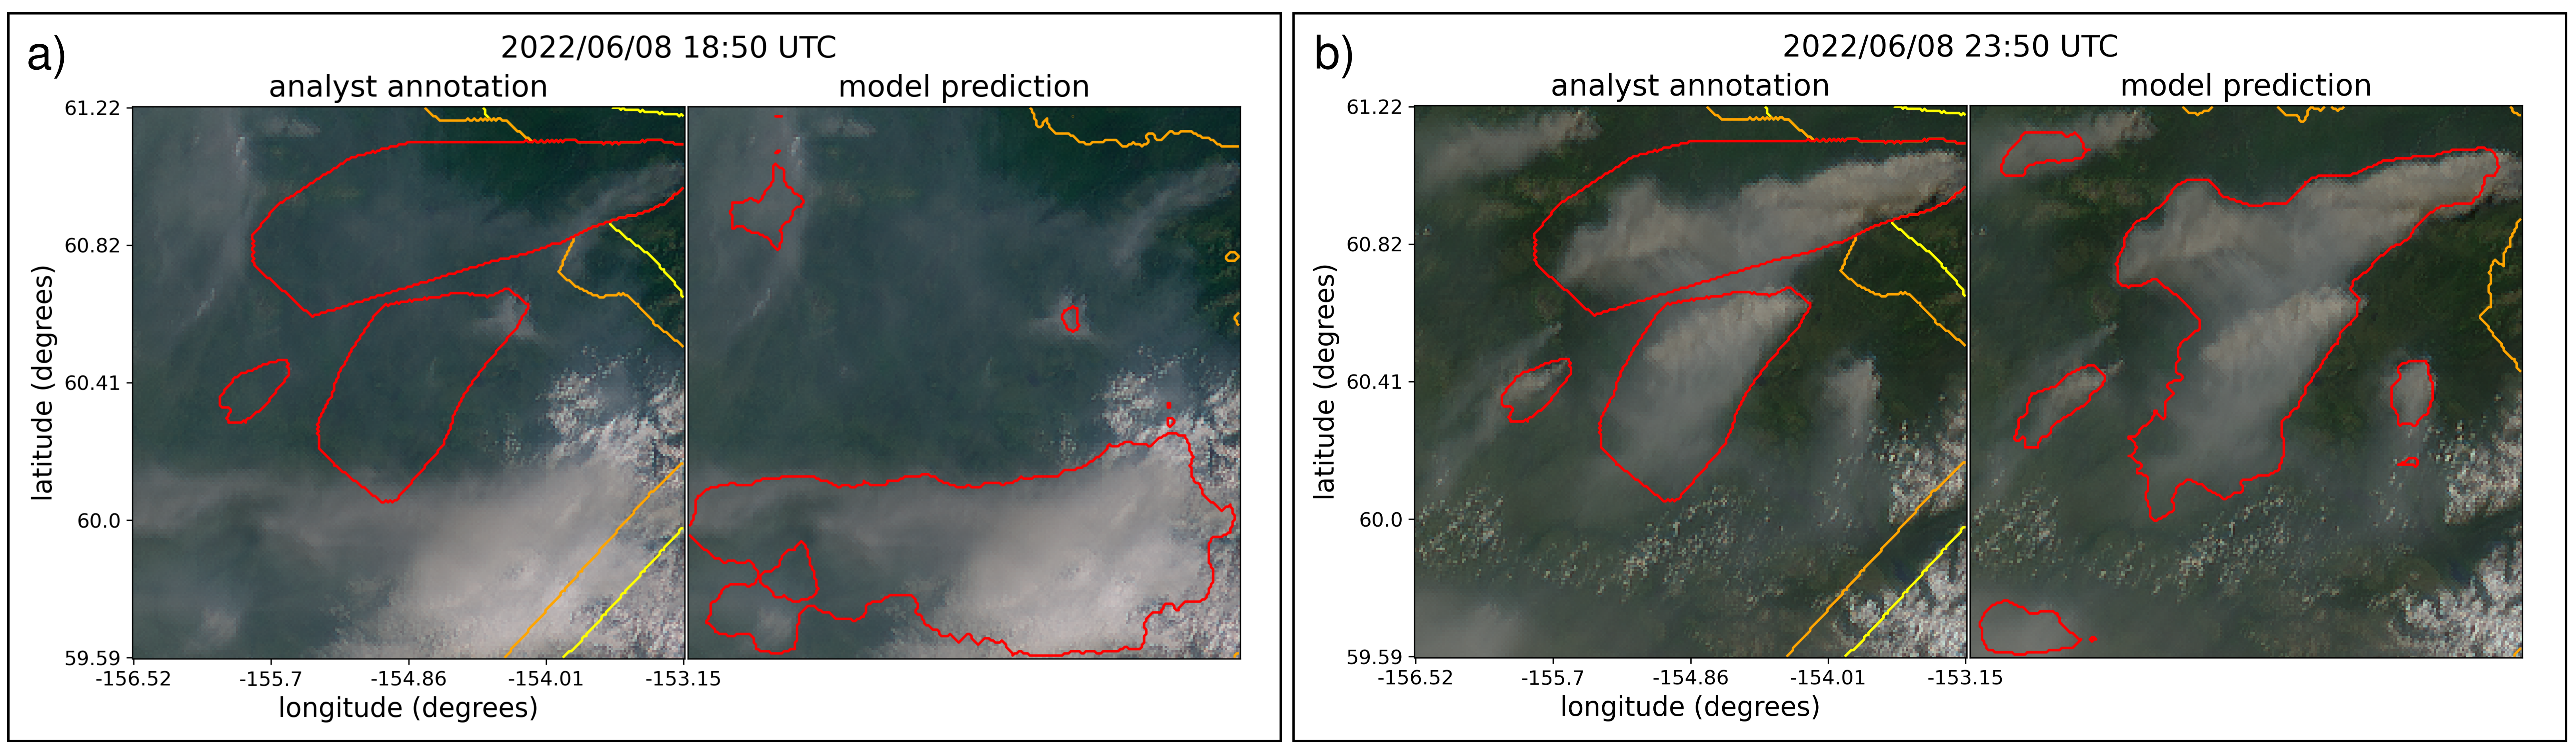
\includegraphics[width=14cm]{figures/D_m_vs_D_pl.png}
    \caption{GOES-West imagery showing smoke on June 8th, 2022 in Alaska where, at this geolocation, daylight was between 12:43-7:53 UTC. The HMS smoke annotations displayed span from 18:50 to 23:50 UTC. a) shows the imagery that was selected using the Mie-derived data selection process b) shows the image that had the highest IoU score between the \(f_p\) generated pseudo-label and the analyst annotation.}\label{ml_vs_mei}
\end{figure}

An illustration of a pseudo-label picked image better representing the analyst annotation when compared to the Mie-derived image selection is evident in Figure \ref{ml_vs_mei}, where the heavy density smoke IoU increases from 0.01 to 0.59. The analyst annotation for these densities cover 5 hours of imagery, the Mie-derived selection optimizes for the image closest to sunrise while the pseudo-label image selection chooses the image with the highest overlap between the pseudo-label and the analyst annotation. 

\section{Limitations}

One of the concerns that comes with using pseudo-labeling methods is that you can perpetuate biases from the parent model into subsequent child models. Due to the increase in detectable forward scattered light off smoke particular matter, we expect the model to have a bias towards producing a higher success rate for smoke detection at larger solar zenith angles. This could potentially cause poor model performance when monitoring smoke during the middle of the day.

\section{Conclusion}

In this study, we have refined an existing dataset originally curated by NOAA's HMS team, transforming it from a many-to-one imagery-to-annotation format to a more succinct, one-to-one satellite image-to-annotation dataset. The initial HMS dataset primarily provided a general approximation of where smoke had been present for a given time window, though it did not guarantee the actual existence of smoke in the labeled pixels during the given times. Our goal was to create a dataset that could be used, along with additional applications, to train a model to detect wildfire smoke in real-time on an image-by-image level. The Mie-derived dataset selection process determines that if smoke is present, what timestamp within the analyst time window would the give the highest smoke signal-to-noise ratio. While optimizing for being able to detect smoke, if it is present, the Mie-dataset selection had no metric to determine if the smoke was effectually present in the selected image. Since many of the images within the HMS time-window either contained no smoke at all or the smoke was not contained within the geospatial bounds of the annotations, the Mie-derived dataset contained a large number of mislabeled samples. Discrepancies between data and labels can be detrimental towards the model's capacity to improve on feature representations in the target domain. During model training, the penalization of accurate predictions can inadvertently introduce biases towards misclassifying noise as meaningful signal. 

To improve the dataset's capacity to accurately represent wildfire smoke plumes, we train a parent machine learning model, \(f_p\),  using the Mie-derived dataset, \(\mathcal{D}_M\), and run it on the relevant satellite images within the time-frame. The image with the maximum IoU score between the model's smoke predictions, or pseudo-label, and the analyst smoke annotations are used to create the pseudo-label generated dataset, \(\mathcal{D}_{PL}\). We then train a child model, \(f_c\), using \(\mathcal{D}_{PL}\) and test \(f_p\) and \(f_c\) on both the 2022 testing sets from \(\mathcal{D}_{M}\) and \(\mathcal{D}_{PL}\). The results reported in table \ref{iou_results} suggest that \(\mathcal{D}_{PL}\) was able to train a better performing model, \(f_c\) that gave higher IoU metrics on both dataset's testing sets in comparison to the original parent model, \(f_p\).

The result of this study is a representative dataset that can be used to train machine learning models for various wildfire smoke applications. A future goal is to produce a robust and reliable machine learning based approach for detecting wildfires using satellite imagery. That information can be used for wildfire monitoring and as data provided to public health officials for air quality assessments. On a broader scale, we show how pseudo-labeling can be used to optimize a dataset when the resolution for the data and corresponding labels do not match. This could be useful in similar applications involving time-series/video data with a singular label where the data can be compressed while still remaining representative of the label. 

\section{Acknowledgments and Disclosure of Funding}

This research was supported in part by NOAA cooperative agreement NA22OAR4320151, for the Cooperative Institute for Earth System Research and Data Science (CIESRDS). We thank Wilfrid Schroeder and the Hazard Mapping Systems team for giving guidance on how they created their smoke plume dataset. This work utilized the Alpine high performance computing resource at the University of Colorado Boulder. Alpine is jointly funded by the University of Colorado Boulder, the University of Colorado Anschutz, Colorado State University, and the National Science Foundation (award 2201538). The statements, findings, conclusions, and recommendations are those of the author(s) and do not necessarily reflect the views of NOAA or the U.S. Department of Commerce. 

\bibliography{references}

\end{document}
